\section{ROS} \label{sec:ros}
El sistema operativo para robots, conocido como ROS (Robot Operating System), se basa en una arquitectura de software distribuida que permite a los diferentes componentes de un robot —como sensores, actuadores y módulos de procesamiento— comunicarse de manera eficiente y flexible. La imagen presentada ilustra de forma clara cómo se lleva a cabo esta comunicación dentro de ROS, mediante el uso de nodos, temas y servicios.

\begin{figure}[h]
	\centering
	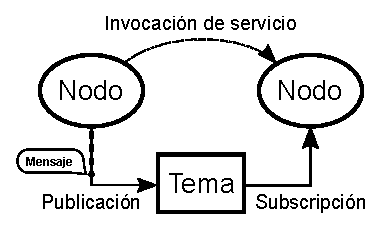
\includegraphics[width=0.5\linewidth]{img/ROS_concepts}
	\caption{Diagrama de comunicación de ROS}
	\label{fig:rosconcepts}
\end{figure}


\subsection{Nodo (Node)}
En el contexto de ROS (Robot Operating System), un nodo es una unidad fundamental de ejecución. Es, básicamente, un proceso independiente que se encarga de realizar una función específica dentro del sistema robótico. Un nodo puede ejecutar una tarea simple, como leer un sensor o mover una articulación, o tareas más complejas como realizar cálculos de trayectoria, procesar imágenes o tomar decisiones autónomas.
Un nodo como componente modular es una de las grandes ventajas de ROS es su arquitectura modular. Esta modularidad se logra dividiendo el sistema robótico en múltiples nodos, donde cada uno realiza una función única y especializada. Gracias a esto, el desarrollo de software se vuelve más organizado y flexible. Si un nodo falla o necesita mejoras, puede modificarse o reiniciarse sin afectar directamente a los demás nodos. Por ejemplo.

\begin{itemize}
    \item Un nodo de sensores puede estar constantemente leyendo datos de un sensor ultrasónico o una cámara.
    \item Un nodo de control puede estar calculando las señales necesarias para mover un motor basado en esos datos.
    \item Un nodo de navegación puede estar trazando rutas o evitando obstáculos.
\end{itemize}



\subsection{Tema (Topic)}
\subsection{Mensaje (Message)}
\subsection{Servicio (Service)}
\subsection{Gazebo}
\subsection{RViz}
